In most of these applications, around 150 features were used to train our machine learning algorithms.  Features were either measured from the learnAir system or harvested from the Forecast.IO weather API.  A few additional features (the EPA reference Black Carbon measurements and Wind Speed and Wind Direction measurements) were all included as training features.  Raw sensor signals are included as well as their calibrated versions.  Many of these signals were further manipulated or processed to give more derived features.  

The measured set of features represents data collected from on-board sensors-- temperature, humidity, noise, light, vibration, pressure/airflow, and other air pollution sensors.  We include the signal from the sensor whose quality we're trying to predict as well (if it reads in certain ranges or slews at a certain rate, we may be able to assume that the sensor is out of its useful range).  

For most of the main features, we created derivative features to capture inaccuracies that may come with too rapid a change in environmental conditions (which anecdotally, we know to be true for electrochemical sensors).  We also looked at intelligently chosen averages over time- ones that helped minimize quantization errors, helped smooth data to match the EPA reference, or whose averaging gave evidence of longer term trends that might also be important in analyzing sensor state and measurement quality.

\begin{marginfigure}
 	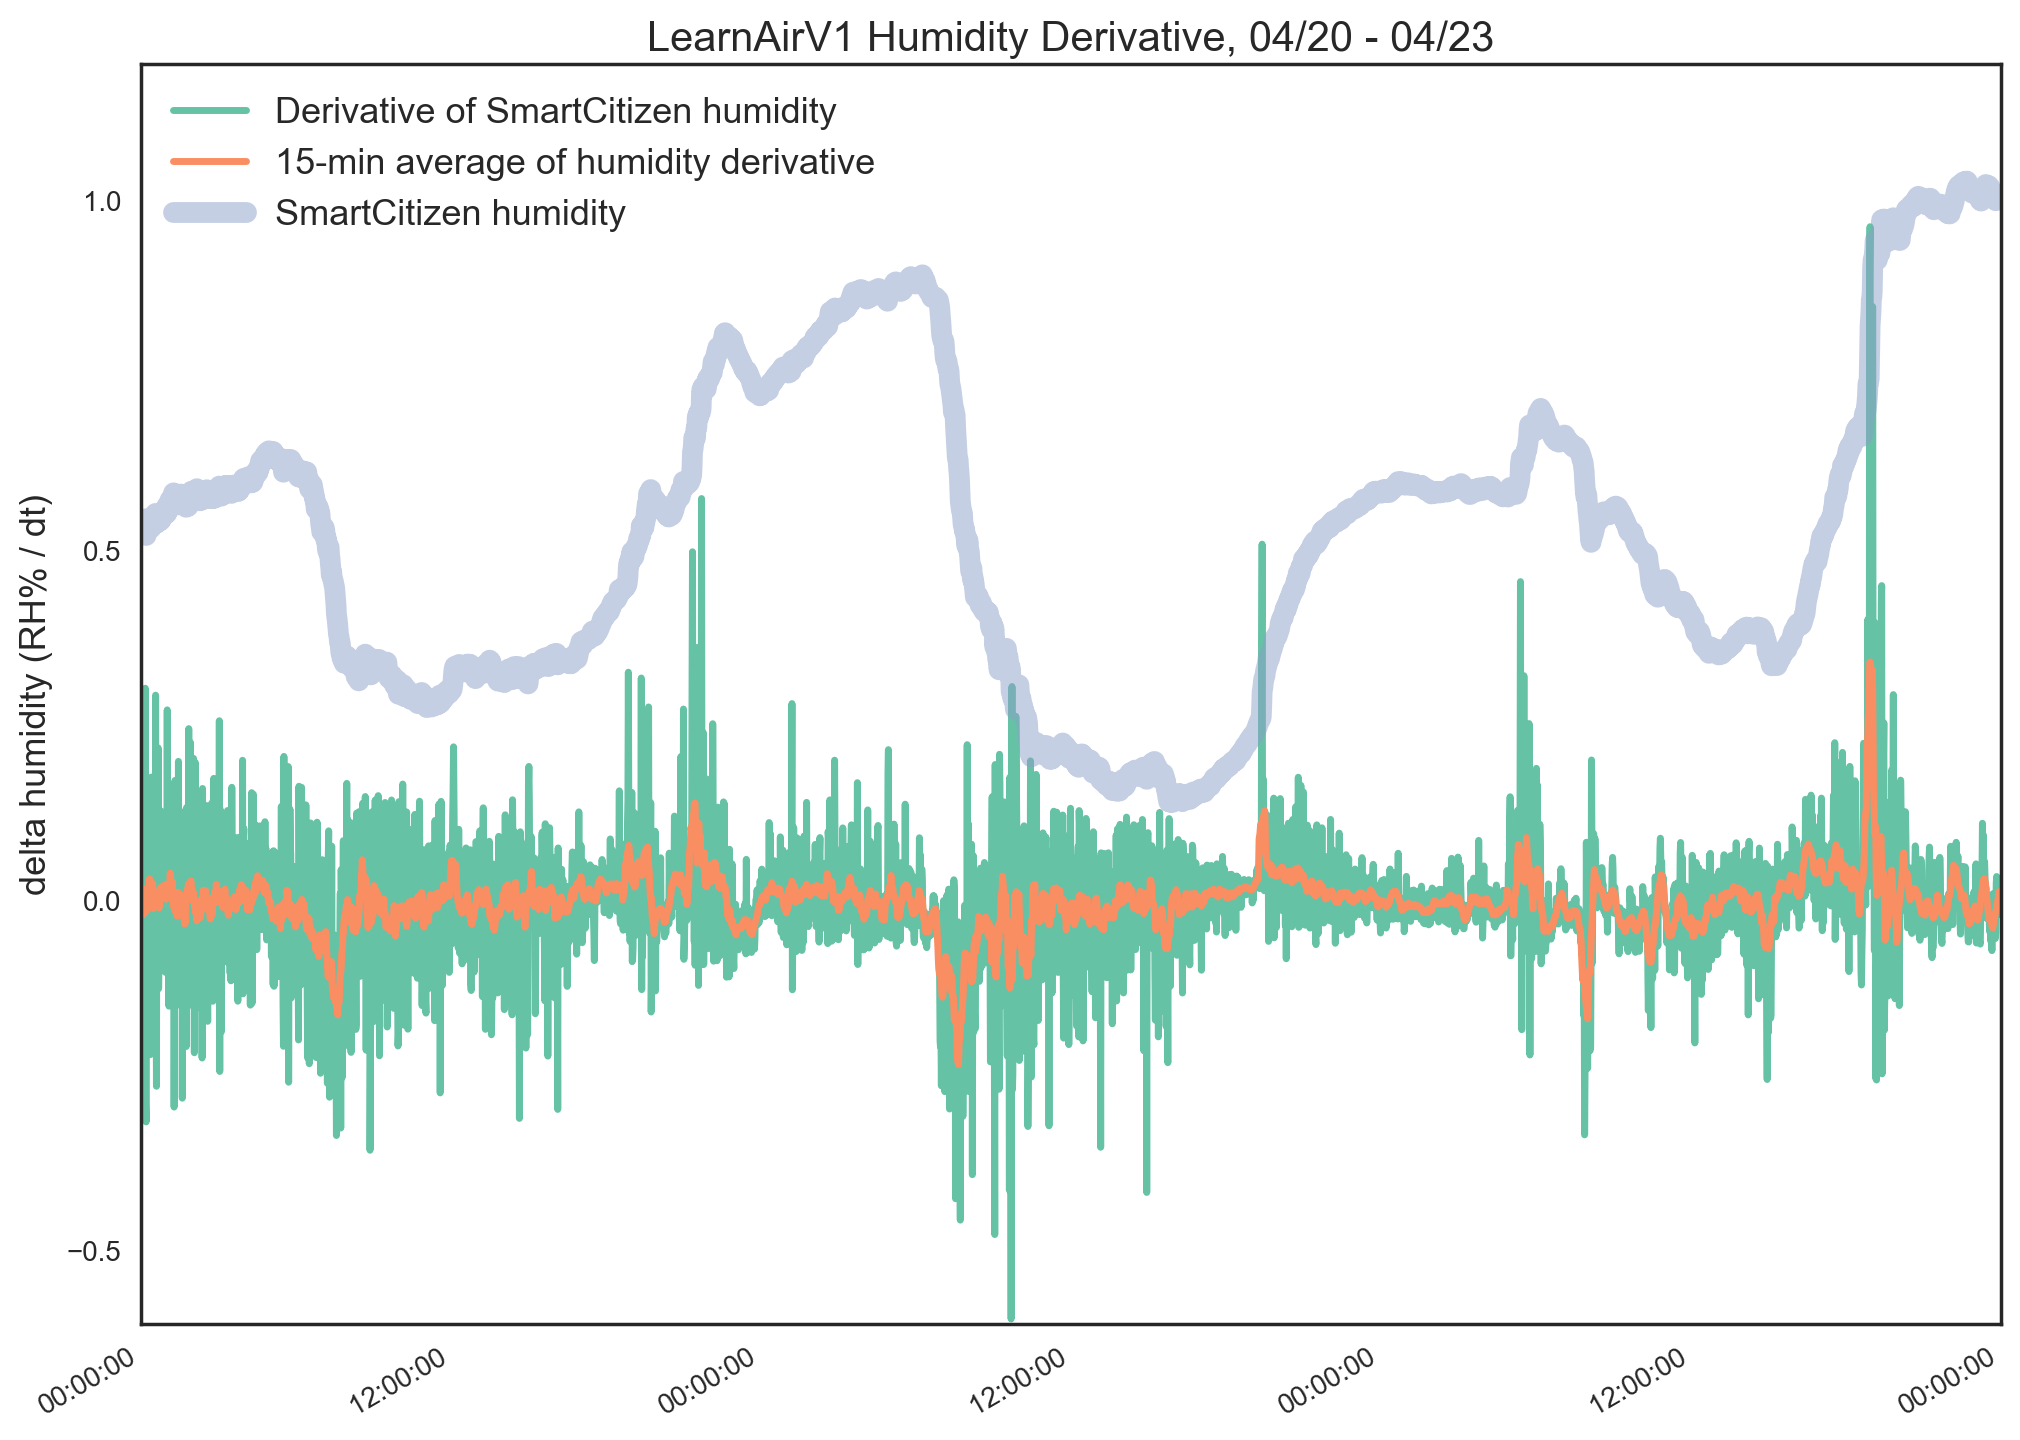
\includegraphics[width=\textwidth]{figs/humidity_derivative}               
 	 \caption{Humidity Derivative Feature Creation}
  	\label{fig:humidity_derivative}
\end{marginfigure}

\begin{figure}[htb]
 	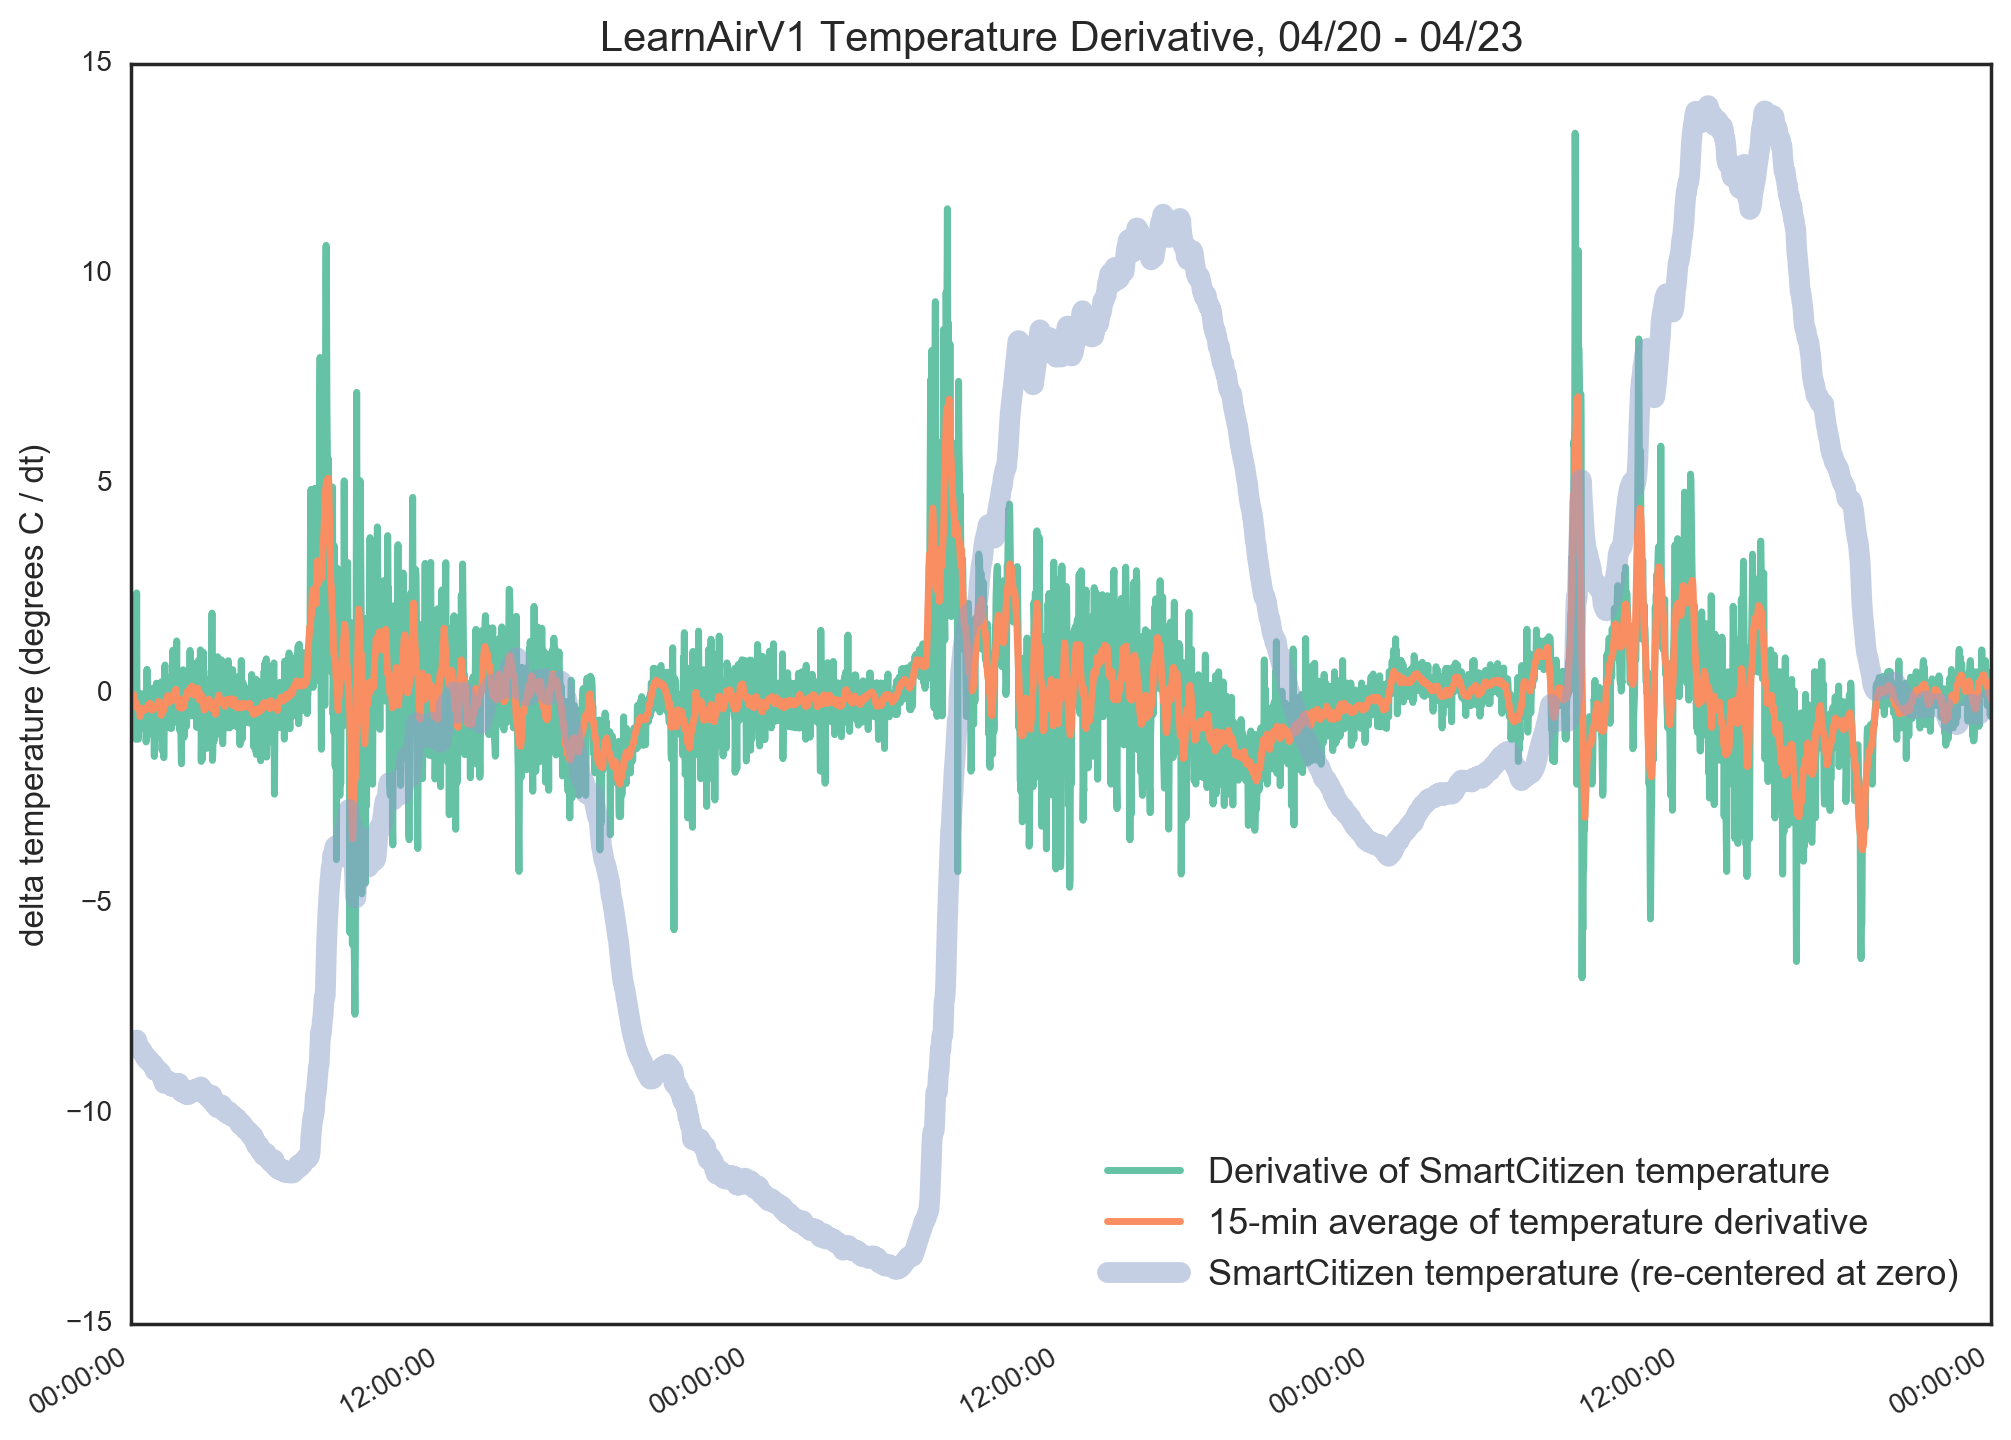
\includegraphics[width=\textwidth]{figs/temp_derivative}               
 	 \caption{Temperature Derivative Feature Creation}
  	\label{fig:temp_derivative}
\end{figure}



Several API's were evaluated for use in this project, and Forecast.IO stood out as a well-reputed option.  They use machine learning to combine many weather forecast APIs into one highly accurate dataset.  The Forecast.IO data comes in hourly intervals, so a running 60 minute average was used to interpolate the values to minute resolution (most of the measured fields, like temperature, are relatively slow-moving, so this technique seems to work).  For class based indicators (for instance, the `weather-summary' field indicating `cloudy', `windy', `foggy', `rainy', etc) we processed the API data as several binary fields.   

Create differential measurements compare measured with API- temp in the box vs. out of the box, as well as humidity in the box vs. out of the box.

\begin{figure}[htb]
 	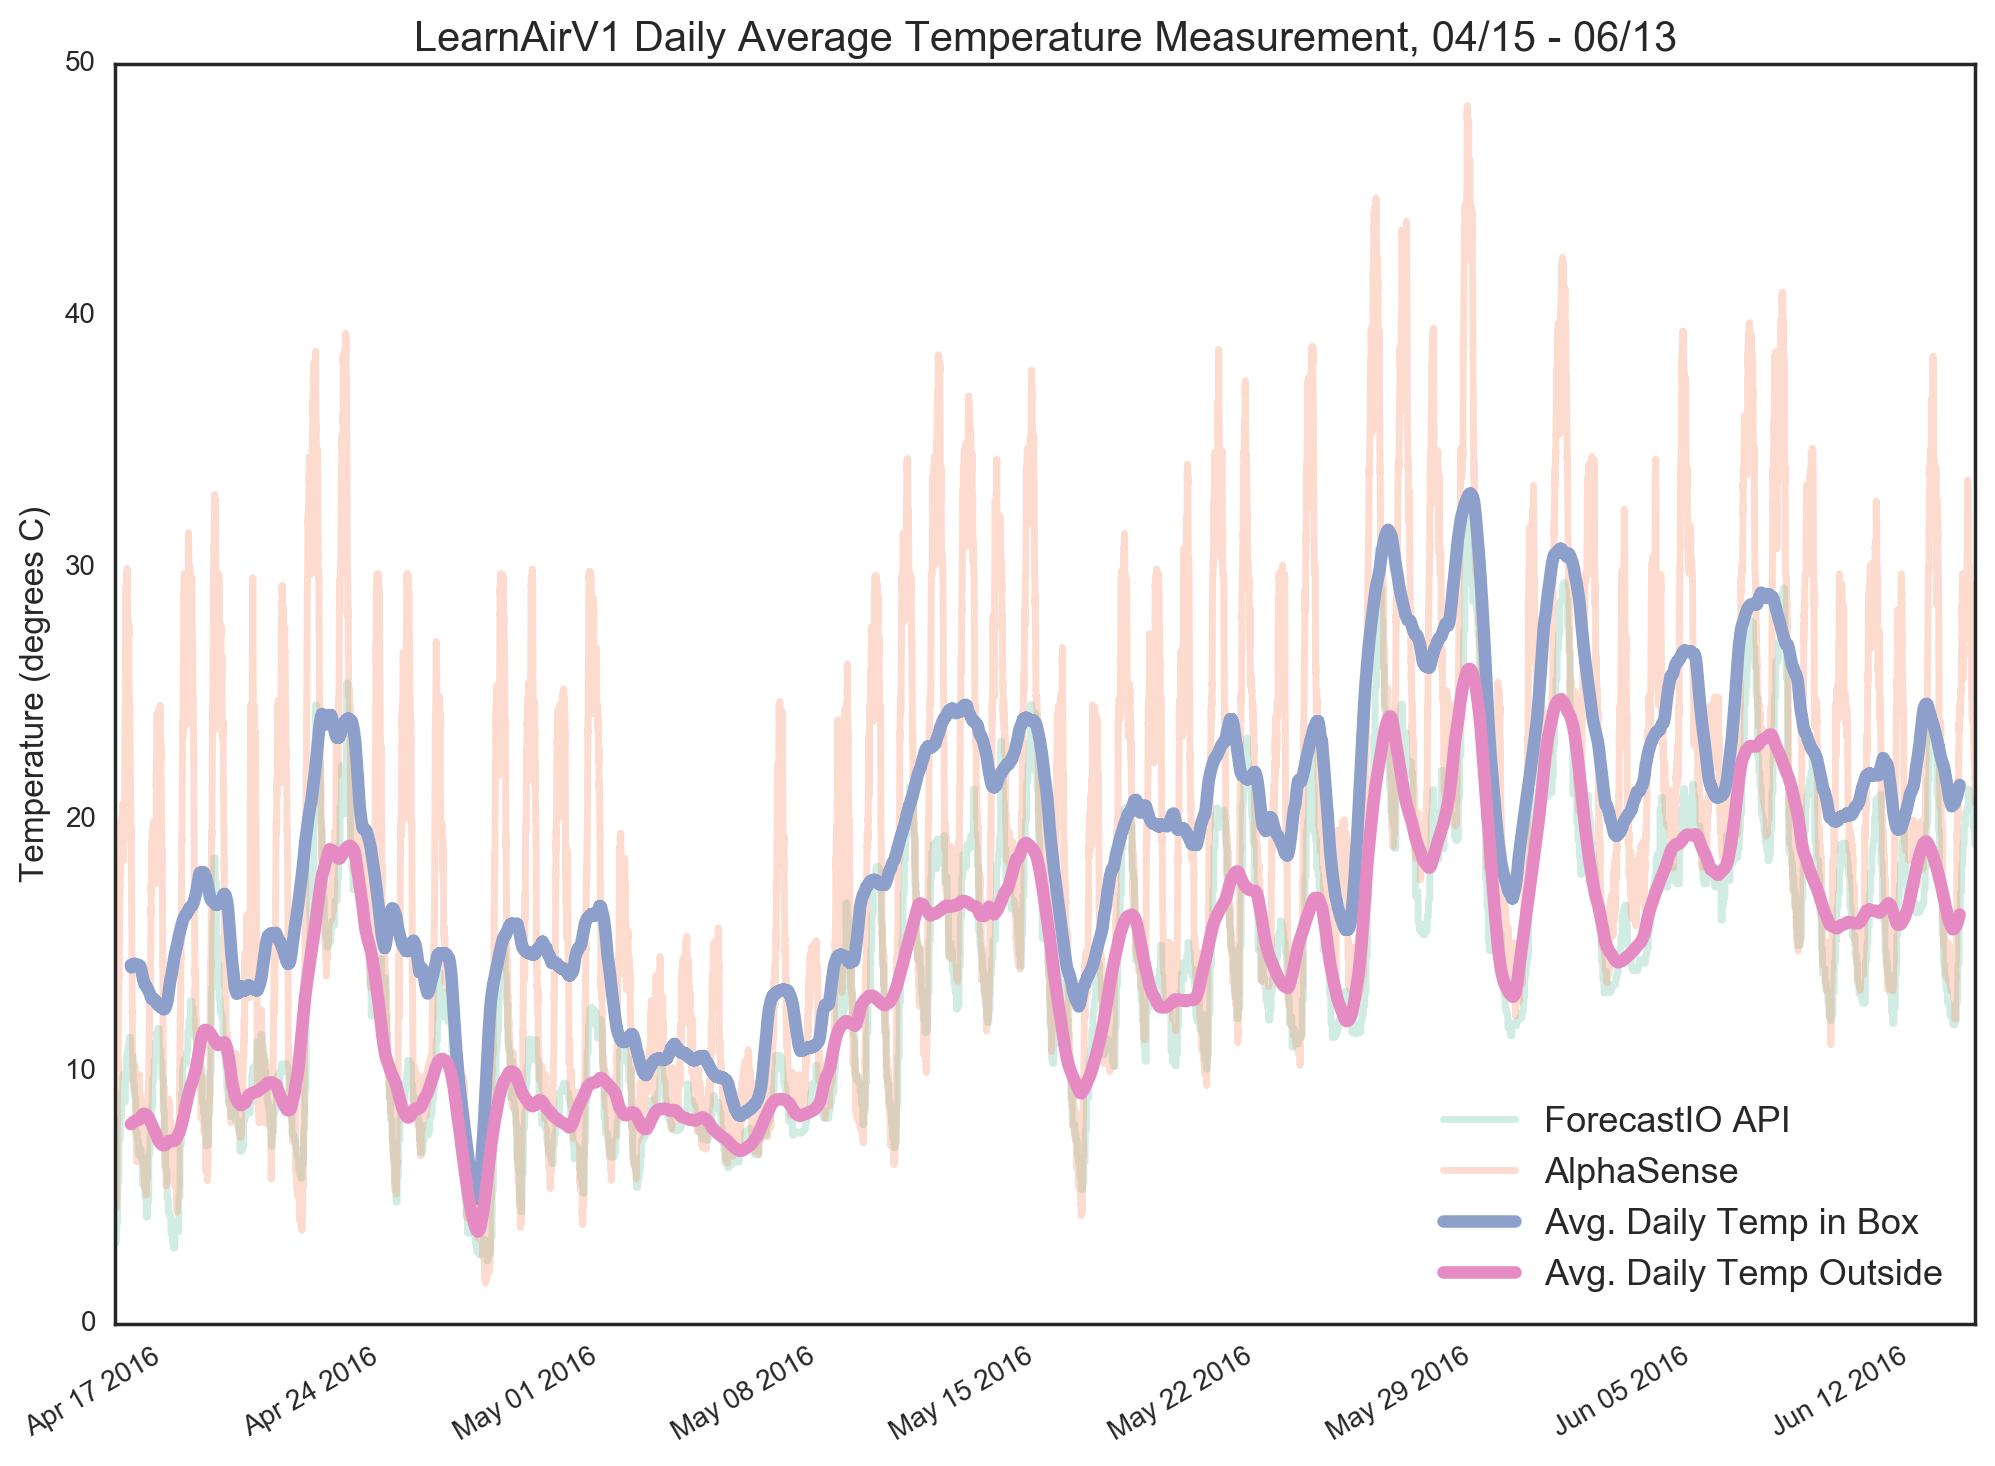
\includegraphics[width=\textwidth]{figs/temp_daily}               
 	 \caption{Temperature during Test Period}
  	\label{fig:temp_daily}
\end{figure}

\begin{figure}[htb]
 	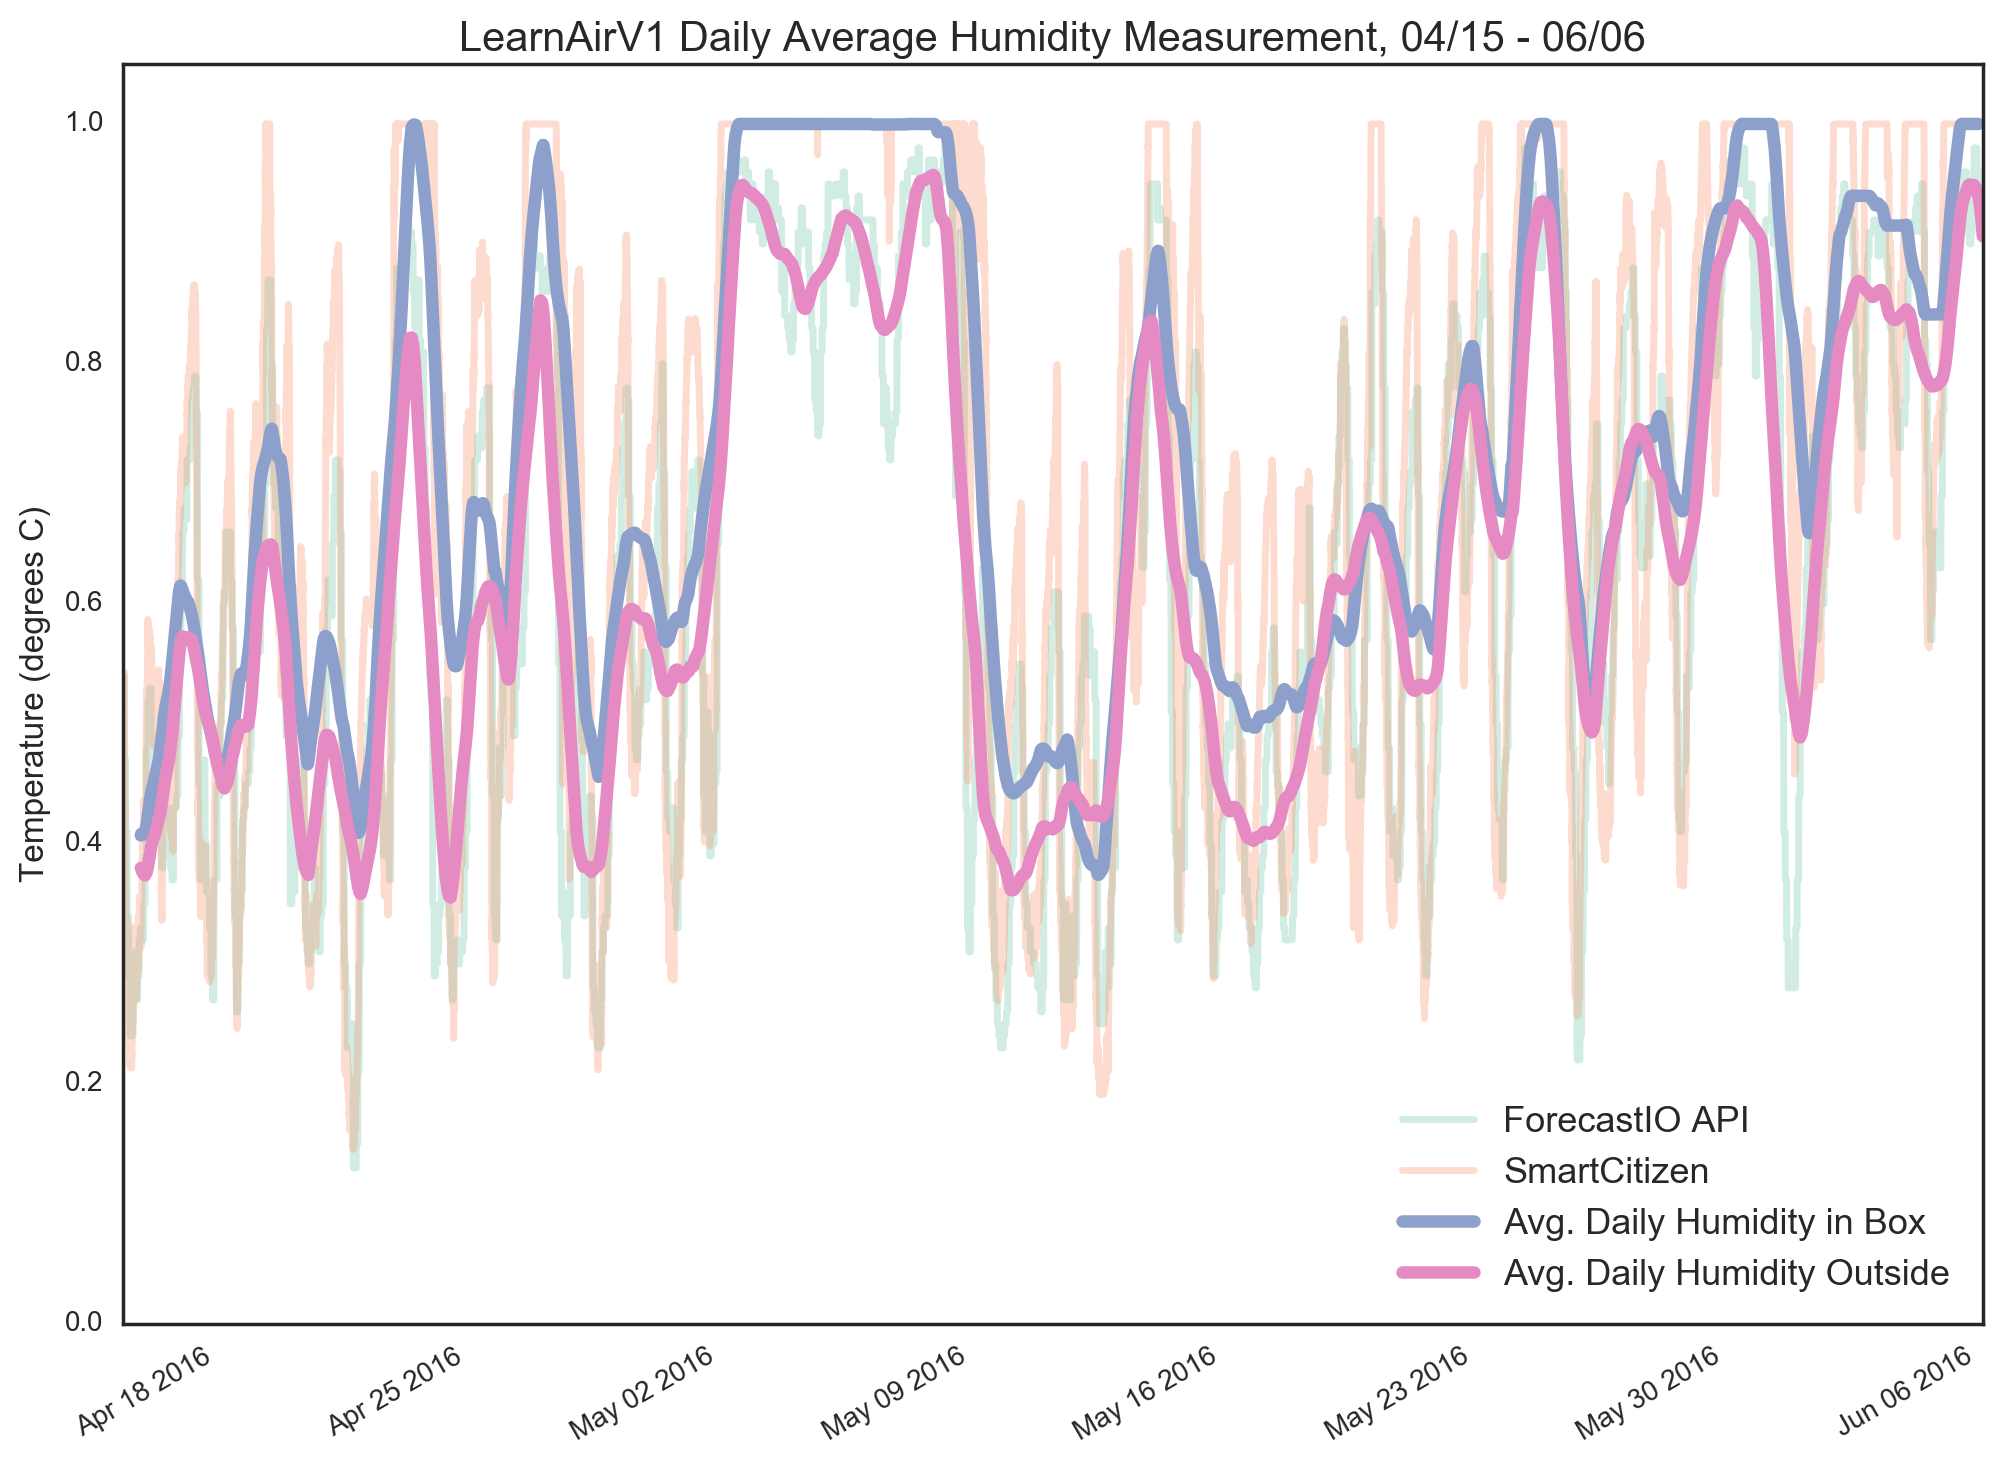
\includegraphics[width=\textwidth]{figs/humidity_daily}               
 	 \caption{Humidity during Test Period}
  	\label{fig:humidity_daily}
\end{figure}

In general, some small subset of features was removed for each training session.  For instance, the higher quality Alphasense CO sensor was removed as a feature when training the less capable SmartCitizen CO sensor.  Training with this feature gives incredibly high accuracy at predicting failure, because it is effectively training itself with the answer.  By training with comparable or cheaper sensors, we can assess the likelihood of a cheap system working predictably.

In most cases, the EPA reference black carbon sensor data was left as a feature- while this is not feasible as a portable, cheap sensor, if this figures prominently in determining a sensor's failure, we can infer something about how the sensor is failing, and what type of sensor we might want to pair it with.  In this way, the machine learning process is not evaluative of a current system's success-- instead, it works as an exploratory tool that might inform a potential system design.

The next page includes a list of the main features.  Processed, calibrated, and other derived features extend this list to the complete.  For histogram plots of many of the main features (made using Weka), see Appendix D.

\begin{table}[H]
\small
\centering
\begin{tabular}{lclc|c|}
\\
\\
\toprule
Feature & Type & Description \\
\midrule
AlphaSense \#1 Work Electrode & Continuous & raw signal from alphasense sensor \\
AlphaSense \#1 Aux Electrode & Continuous & raw signal from alphasense sensor \\
AlphaSense \#2 Work Electrode & Continuous & raw signal from alphasense sensor \\
AlphaSense \#2 Aux Electrode & Continuous & raw signal from alphasense sensor \\
AlphaSense \#3 Work Electrode & Continuous & raw signal from alphasense sensor \\
AlphaSense \#3 Aux Electrode & Continuous & raw signal from alphasense sensor \\
AlphaSense O3 & Continuous & calibrated signal from raw electrode readings \\
AlphaSense NO2 & Continuous & calibrated signal from raw electrode readings \\
AlphaSense CO & Continuous & calibrated signal from raw electrode readings \\
AlphaSense H2S & Continuous & calibrated signal from raw electrode readings \\
AlphaSense Temperature & Continuous & raw signal from alphasense temp sensor \\
Wind Pressure Reading & Continuous & raw signal from pressure sensor \\
Corrected Wind Reading & Continuous & conditioned pressure signal to relate to wind \\
Sharp Dust Reading & Continuous & raw signal from optical particulate sensor \\
SmartCitizen CO Voltage & Continuous & raw signal from smartCitizen CO sensor \\
SmartCitizen NO2 Voltage & Continuous & raw signal from smartCitizen NO2 sensor \\
SmartCitizen Noise Voltage & Continuous & raw signal from smartCitizen Piezo mic \\
SmartCitizen Humidity Voltage & Continuous & raw signal from smartCitizen SHT15 \\
SmartCitizen Temperature Voltage & Continuous & raw signal from smartCitizen SHT15 \\
SmartCitizen Humidity & Continuous & conditioned smartCitizen Humidity Measurement \\
SmartCitizen Temperature & Continuous & conditioned smartCitizen Temperature Measurement \\
SmartCitizen Light Reading & Continuous & raw signal from smartCitizen light sensor \\
SmartCitizen Solar Panel Charge & Continuous & raw signal from smartCitizen sensor \\
EPA Sensor Wind Direction & Continuous & calibrated, accurate EPA reference measurement \\
EPA Sensor Wind Speed  & Continuous & calibrated, accurate EPA reference measurement \\
EPA Sensor Black Carbon  & Continuous & calibrated, accurate EPA reference measurement \\
ForecastIO Apparent Temperature & Continuous & calibrated api call measurement \\
ForecastIO Cloud Cover & Continuous & calibrated api call measurement \\
ForecastIO Dew Point & Continuous & calibrated api call measurement \\
ForecastIO Humidity & Continuous & calibrated api call measurement \\
ForecastIO Precipitation Intensity & Continuous & calibrated api call measurement \\
ForecastIO Precipitation Probability & Continuous & calibrated api call measurement \\
ForecastIO Pressure & Continuous & calibrated api call measurement \\
ForecastIO Temperature & Continuous & calibrated api call measurement \\
ForecastIO Visibility & Continuous & calibrated api call measurement \\
ForecastIO Wind Bearing & Continuous & calibrated api call measurement \\
ForecastIO Wind Speed & Continuous & calibrated api call measurement \\
ForecastIO Clear Night & Boolean & calibrated api call measurement \\
ForecastIO Clear Day & Boolean & calibrated api call measurement \\
ForecastIO Partly Cloudy Day & Boolean & calibrated api call measurement \\
ForecastIO Partly Cloudy Night & Boolean & calibrated api call measurement \\
ForecastIO Cloudy & Boolean & calibrated api call measurement \\
ForecastIO Rainy & Boolean & calibrated api call measurement \\
ForecastIO Foggy & Boolean & calibrated api call measurement \\
ForecastIO Windy & Boolean & calibrated api call measurement \\
Morning Hours & Boolean & created field to correspond to the morning \\
Afternoon Hours & Boolean & created field to correspond to the afternoon \\
Evening Hours & Boolean & created field to correspond to the evening \\
Morning Rush Hours & Boolean & created field to correspond to the morning rush \\
Lunch Hours & Boolean & created field to correspond to the lunch \\
Evening Rush Hours & Boolean & created field to correspond to the evening rush \\
Day Hours & Boolean & created field to correspond to the day \\
Night Hours & Boolean & created field to correspond to the night \\
Outside and Inside Box Temp Differential & Continuous & Difference between temp out/in box \\
Minutes Since Plugged In & Continuous & to help quantify initial terrible readings as sensor settles \\
Day of Year & Continuous & day resolution proxy for seasonality \\
\bottomrule
\end{tabular}
\label{tab:feature_table}
\caption{Machine Learning Features used to Predict Sensor Accuracy}
\end{table}


